\documentclass[runningheads]{llncs}
\def\shownotes{1}
\def\notesinmargins{0}

%\usepackage{fullpage}
\usepackage{fancyvrb}
\usepackage{mathtools,color,xcolor,hyperref,graphicx,wrapfig,listings,array,xspace}
\usepackage{caption}
\usepackage{subcaption}
\usepackage{tikz}
\usetikzlibrary{arrows}

\usepackage{amsfonts}
% https://tex.stackexchange.com/questions/11719/how-do-i-backcolor-in-verbatim
\usepackage{xcolor}
\usepackage{alltt}
% Compensate for fbox sep:
\newcommand\Hi[2][lightgray]{%
	\hspace*{-\fboxsep}%
	\colorbox{#1}{#2}%
	\hspace*{-\fboxsep}%
}

\ifnum\shownotes=1
\ifnum\notesinmargins=1
\newcommand{\authnote}[2]{\marginpar{\parbox{\marginparwidth}{\small %
  \textsf{#1 {\textcolor{blue}{notes: #2}}}}}%
  \textcolor{blue}{\textbf{\dag}}}
\else
\newcommand{\authnote}[2]{
  \textsf{#1 \textcolor{blue}{: #2}}}
\fi
\else
\newcommand{\authnote}[2]{}
\fi

\newcommand{\snote}[1]{{\authnote{\textcolor{yellow}{Scalahub notes}}{#1}}}
\newcommand{\knote}[1]{{\authnote{\textcolor{green}{kushti notes}}{#1}}}


\newcommand{\ret}{\mathsf{ret}}
\newcommand{\new}{\mathsf{new}}
\newcommand{\hnew}{h_\mathsf{new}}
\newcommand{\old}{\mathsf{old}}
\newcommand{\op}{\mathsf{op}}
\newcommand{\verifier}{\mathcal{V}}
\newcommand{\prover}{\mathcal{P}}
\newcommand{\key}{\mathsf{key}}
\newcommand{\nextkey}{\mathsf{nextKey}}
\newcommand{\node}{\mathsf{t}}
\newcommand{\parent}{\mathsf{p}}
\newcommand{\leaf}{\mathsf{f}}
\newcommand{\vl}{\mathsf{value}}
\newcommand{\balance}{\mathsf{balance}}
\newcommand{\lft}{\mathsf{left}}
\newcommand{\rgt}{\mathsf{right}}
\newcommand{\lbl}{\mathsf{label}}
\newcommand{\direction}{\mathsf{d}}
\newcommand{\oppositedirection}{\bar{\mathsf{d}}}
\newcommand{\found}{\mathsf{found}}
\newcommand{\mypar}[1]{\smallskip\noindent\textbf{#1.}\ \ \ }
\newcommand{\ignore}[1]{}

\newcommand{\langname}{ErgoScript\xspace}
\newcommand{\powname}{Autolykos\xspace}
\newcommand{\poolname}{ErgoPool\xspace}
\newcommand{\mixname}{ErgoMix\xspace}


\newcommand{\lst}[1]{\text{\lstinline[basicstyle={\ttfamily}]$#1$}}

\newcommand{\andnode}{\ensuremath{\mathsf{AND}}}
\newcommand{\ornode}{\ensuremath{\mathsf{OR}}}
\newcommand{\tnode}{\ensuremath{\mathsf{THRESHOLD}}}

\newcommand{\primname}{Commitment of Work\xspace}
\newcommand{\prim}{CoW\xspace}


\newcommand{\GF}{\ensuremath{\mathrm{GF}}}


\begin{document}

\newcommand{\algname}{ZeroJoin\xspace}
\title{\algname: Combining ZeroCoin and CoinJoin}

\author{Alexander Chepurnoy\inst{1,2}, Amitabh Saxena\inst{1}}

\institute{Ergo Platform \\\email{\{kushti\}@protonmail.ch, \{amitabh123\}@gmail.com} \and
IOHK Research \\\email{\{alex.chepurnoy\}@iohk.io}}

\maketitle

\begin{abstract}

We present \algname, a practical privacy-enhancing protocol for blockchain transactions. \algname can be considered a combination of ZeroCoin and CoinJoin. It borrows ideas from both but attempts to overcome some of their drawbacks.
Like ZeroCoin, our protocol uses zero-knowledge proofs and a pool of
participants. However, unlike ZeroCoin, our proofs are very efficient, and our pool size is not monotonically increasing.
Thus, our protocol overcomes the two major drawbacks of ZeroCoin. Our approach can also be considered a non-interactive variant of CoinJoin, where the interaction is replaced by a public transaction on the blockchain. The security of \algname is based on the Decision Diffie-Hellman (DDH) assumption. 
We also present \mixname, a practical implementation of \algname on top of Ergo, a smart contract platform based on Sigma protocols. While \algname contains the key ideas, it leaves open the practical issue of handling fees. The key contribution of \mixname is a novel approach to handle fee in \algname. 

\end{abstract}

\section{Introduction}
\label{intro}

Privacy enhancing techniques in blockchains generally fall into two categories. The first is hiding the amounts being transferred, such as in Confidential Transactions~\cite{ct}. The second is obscuring the input-output relationships such as in ZeroCoin~\cite{zerocoin}, CoinJoin~\cite{coinjoin}. Some solutions such as MimbleWimble~\cite{mw} and Zcash~\cite{zcash,zcash1} combine both approaches.
%In fact, MW can be thought of as a combination of CT and OWAS.

In this work, we describe \algname, another privacy enhancing protocol based on the latter approach of obscuring the input-output relationships, while keeping the amounts public. This allows us to avoid expensive range proofs necessary for the first approach. Our protocol is motivated from ZeroCoin and CoinJoin in order to overcome some of their limitations, and can be thought of as a combination of the two.


\section{Background}

Bitcoin~\cite{Nak08}, ZeroCoin~\cite{zerocoin}, Zcash~\cite{zcash} and Ergo~\cite{ergo} are based on the idea of ``coins'' which are short-lived immutable data structures, often called UTXOs (short for {unspent transaction outputs}). \algname also uses UTXOs. 

\subsection{UTXO Blockchains}
In UTXO-based blockchains, every node maintains an in-memory database of all current UTXOs, called the {\em UTXO-set}. A transaction consumes (destroys) some UTXOs and creates new ones. When a node receives a block, it updates its UTXO-set based on the transactions in that block. A UTXO is a single-use object, and its simplest form contains a public key (in which case, the UTXO can be ``spent'' using the corresponding private key). Spending a UTXO essentially involves executing any embedded code inside it and removing it from the UTXO-set. UTXOs can be likened to physical coins, which get passed around between people and one person may hold multiple coins at any time (one private key can control multiple unspent UTXOs). 
The alternative to UTXOs is the {\em account}-based model of Ethereum~\cite{wood2014ethereum}. Unlike UTXOs, accounts are long-lived and mutable. Each private key controls exactly one account, which can be likened to real-world bank accounts. While a UTXO must be completely spent (i.e., its balance cannot be changed), an account at the bare minimum allows changing the balance. Most privacy techniques including CoinJoin and ZeroCoin are designed for UTXOs and cannot be easily adapted for accounts. Our protocol also works in the UTXO model only. %and leaks information if used in the account-based model.

\subsection{Guard Scripts}
A UTXO is protected by a {\em guard script}, a computer program encoding a {\em proposition}. The proposition defines the set of conditions that must be satisfied when spending the UTXO. The spender supplies a {\em proof} of satisfying the proposition. For example, the proposition may require that the entire transaction's bytes (sans the proof section) must be signed under some public key. The proof is then the signature on the transaction's bytes generated using the corresponding private key. In fact, this is the most common scenario in all UTXO systems. 
The guard script can encode arbitrarily complex conditions as long as they can be encoded in the underlying language. 
Guard scripts are also called smart contracts. A {\em box} is another name for a UTXO in Ergo~\cite{ergo} and we will use these two terms interchangeably.

\subsection{Execution Context}
\label{context}

In UTXO blockchains, a block contains a compact section called the {\em header}, which is
enough to verify the block solution and check integrity of other sections (such as block transactions). 
The execution context (or simply the context) is the information available to a smart contract during execution. 
To encode \algname in smart contracts (rather than within the protocol), the underlying scripting language must support  a sufficiently rich context.

We can classify the context based on what part of the block a smart contract can access. At the bare minimum, the first level, the smart contract should have access to the contents of the UTXO it guards (i.e., its monetary value and any other data stored in it). At the second level, the smart contract may additionally have access to the entire spending transaction, that is, all its inputs and outputs. At the third level, the smart contract may have access to block header data in addition to the data at the second level. For example, in \langname (which operates at this level), the last ten block headers and part of the next block header that is known in advance are also available in the execution context. Finally, at the fourth level, the execution context may contain the entire block with all sibling transactions. Note that since the execution context must fit into random-access memory of commodity hardware, accessing the full blockchain is not a realistic scenario. The following
 table summarizes possible execution context components.

~\\
\begin{tabular}{|l|l|l|l|l|l|}\hline
	Context level & UTXO & Transaction & Header      & Block & Example \\ \hline
	 C1     & Yes  & No          & No  		   & No    & Bitcoin~\cite{Nak08} \\
	 C2     & Yes & Yes         & No 		   & No    & -- \\
	 C3     & Yes & Yes         & Yes 		   & No    & \langname ~\cite{ergo}   \\
	 C4     & Yes & Yes         & Yes 		   & Yes   & --    \\\hline
\end{tabular}

\subsection{CoinJoin} 
\label{coinjoin}
CoinJoin~\cite{coinjoin} is a privacy enhancing protocol where multiple parties provide inputs and create outputs in a single transaction computed interactively such that the original inputs and outputs are unlinked. The optimal use of CoinJoin is when two inputs of equal value are joined to generate two outputs of equal value, and the process is repeated, as depicted in Figure~\ref{fig:coinjoin}. 

\begin{figure}[h]
	\centering
	\begin{subfigure}{.6\textwidth}
		\centering
		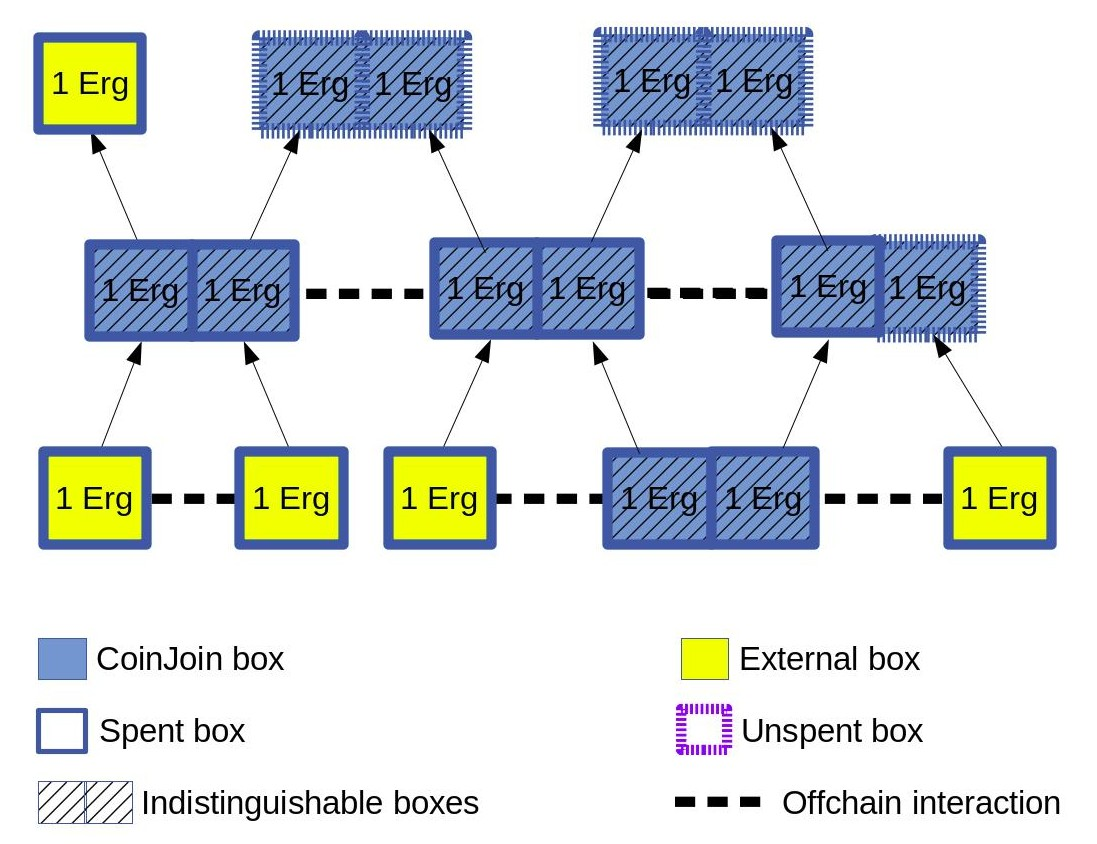
\includegraphics[width=\linewidth]{CoinJoin.jpg}
	\end{subfigure}%
	\caption{Canonical Multi-stage CoinJoin}
	\label{fig:coinjoin}
\end{figure}

In this model, each CoinJoin transaction has exactly two inputs (the boxes at the tail of the arrows) and two outputs (the boxes at the head of the arrows). Creating such a transaction requires a private off-chain interaction between the two parties supplying the inputs, which is denoted by the dashed line. We will ignore fee for now and revisit this issue in Section~\ref{fee}.

The key idea of CoinJoin is that the two output boxes are {\em indistinguishable} in the following sense. 
\begin{enumerate}
    \item The owner of each input box controls exactly one output box.
    \item An outsider cannot guess with probability better than 1/2, which output corresponds to which input.
\end{enumerate}

Thus, each CoinJoin transaction provides 50\% unlinkability. The output box can be used as input to further CoinJoin transactions and the process repeated to increase the unlinkability to any desired level. We will use the same concept in \algname. 
CoinJoin requires two parties to interactively sign a transaction off-chain and this interactive nature is the primary drawback of CoinJoin, which \algname aims to overcome. 

\subsection{ZeroCoin}
\label{zerocoin} 

ZeroCoin is a privacy enhancing protocol depicted in Figure~\ref{fig:zerocoin}. 

\begin{figure}[h]
	\centering
	\begin{subfigure}{.8\textwidth}
		\centering
		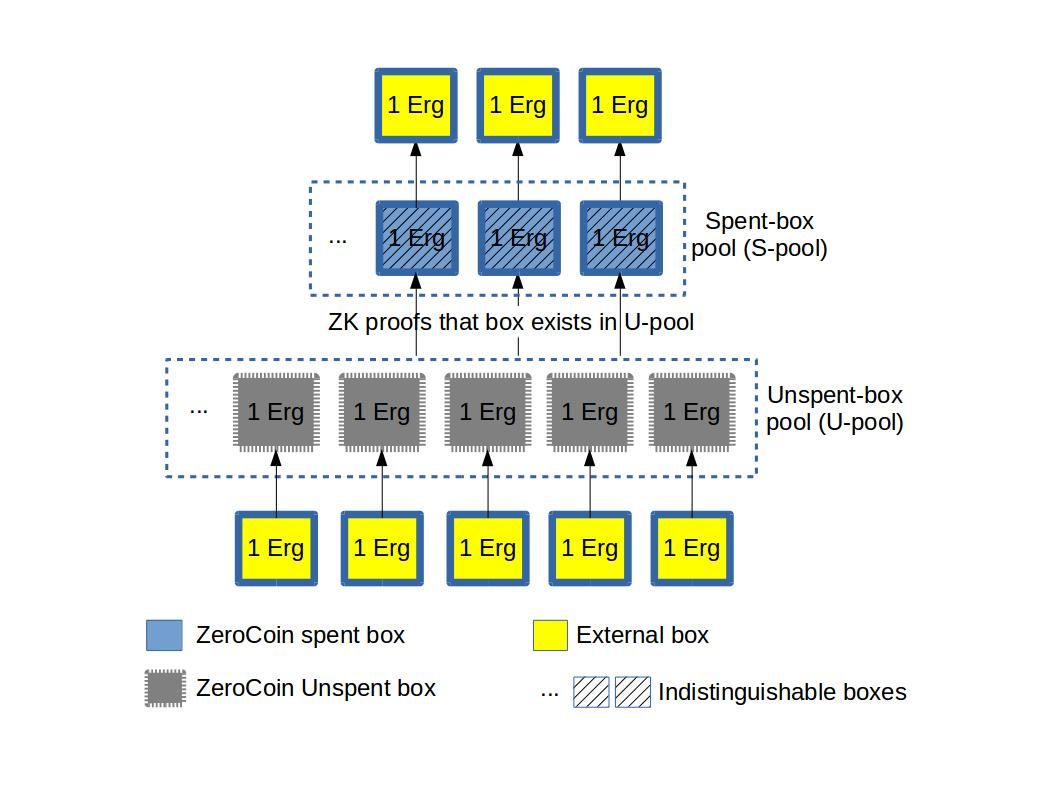
\includegraphics[width=\linewidth]{ZeroCoin.jpg}
	\end{subfigure}
	\caption{ZeroCoin protocol}
	\label{fig:zerocoin}
\end{figure}

The protocol uses a mixing pool (called the {\em unspent-box pool}, or simply the U-pool), to which an ordinary coin is added as a commitment $c$ to secrets $(r, s)$. The coin is later spent such that the link to $c$ is not publicly visible. The value $c$ must be permanently stored in the U-pool, since the spending transaction cannot reveal it. Instead, it reveals the secret $s$ (the {\em serial number}) along with a zero-knowledge proof that $s$ was used in a commitment from the pool. To prevent double spending, the serial number is also stored in another space called the {\em spent-box pool} (the S-pool). A coin can be spent from the U-pool only if the corresponding serial number does not exist in the S-pool. 

One consequence of this is that both the U-pool (the set of commitments) and the S-pool (the set of spent serial numbers) must be maintained in memory for verifying every transaction. 
Another consequence is that the sizes of the these two sets increase monotonically. 
This is the main drawback of ZeroCoin (also ZCash~\cite{zcash}), which \algname tries to address. 
In \algname, once a box is spent, no information about it is kept in memory, and in particular no data sets of monotonically increasing sizes are maintained. 

Considering the addition of a coin to the mix as a deposit and removal as a withdraw, the in-memory storage in \algname is proportional to the number of deposits minus the number of withdraws, while that in ZeroCash is proportional to the number of deposits plus the number of withdraws.  

\subsection{$\Sigma$-Protocols} 

\algname uses two-party interactions called $\Sigma$-protocols defined over a cyclic multiplicative group $G$ of prime order $q$ such that the decision Diffie-Hellman (DDH) problem in $G$ is hard. Specifically, is uses two such protocols. The first, denoted \texttt{proveDlog($u$)}, is a {\em proof of knowledge of Discrete Logarithm} of some group element $u$ with respect to a fixed generator $g$. That is, the prover proves knowledge of $x$ such that $u = g^x$ by using Schnorr signatures~\cite{Sch91}. See Appendix~\ref{intro:sigma} for an overview of the protocol. 

The second primitive, denoted \texttt{proveDHTuple($g, h, u, v$)}, is a {\em proof of knowledge of Diffie-Hellman Tuple}, where the prover proves knowledge of $x$ such that $u = g^x$ {\em and} $v = h^x$ for a arbitrary generators $g$ and $h$. This is essentially two instances of the first protocol running in parallel as follows.

\begin{enumerate}
	\item The prover picks $r \stackrel{R}{\leftarrow} \mathbb{Z}_q$ and computes $(t_0, t_1) = ({g}^r, {h}^r)$. It sends $(t_0, t_1)$ to the verifier.
	\item The verifier picks $c \stackrel{R}{\leftarrow} \mathbb{Z}_q$ and sends $c$ to prover.
	\item The prover sends $z = r + cx$ to the verifier. 
	\item The verifier accepts iff ${g}^z = {t_0}\cdot {u}^c$ and $h^z=t_1\cdot v^c$.
\end{enumerate}

We use the non-interactive variant of the above protocol obtained via the Fiat-Shamir transform, where $c = H(t_0 \Vert t_1\Vert m)$ for some message $m$ to be signed.  Observe that \texttt{proveDHTuple} requires 4 exponentiations for verification, while \texttt{proveDlog} requires 2. 

\langname supports both the protocols, and thus has all the primitives needed to implement \algname.

\section{\algname Protocol}

\algname uses a pool of {\em Half-Mix} boxes, which are boxes ready for mixing. The set of all unspent Half-Mix boxes is called the {\em H-pool}. To mix an arbitrary box $B$, one of the following is done:
\begin{enumerate}
	\item \textbf{Pool:} Add $B$ to the H-pool (by converting it to a Half-mix box) and wait for someone to mix it.
	\item \textbf{Mix:} Pick any box $A$ from the H-pool and a secret bit $b$. Spend $A, B$ to generate two {\em Fully Mixed} boxes $O_0, O_1$ such $O_b$ and $O_{1-b}$ are spendable by $A$'s and $B$'s owners respectively.
\end{enumerate}

Privacy comes from the fact that boxes $O_b$ and $O_{1-b}$ are indistinguishable so an outsider cannot guess $b$ with probability better than 1/2. Thus, the probability of guessing the original box after $n$ mixes is $1/2^n$. A box is mixed several times for the desired privacy. The protocol is depicted in Figure~\ref{fig:mixname}. 

\begin{figure}[h]
	\centering
	\begin{subfigure}{.6\textwidth}
		\centering
		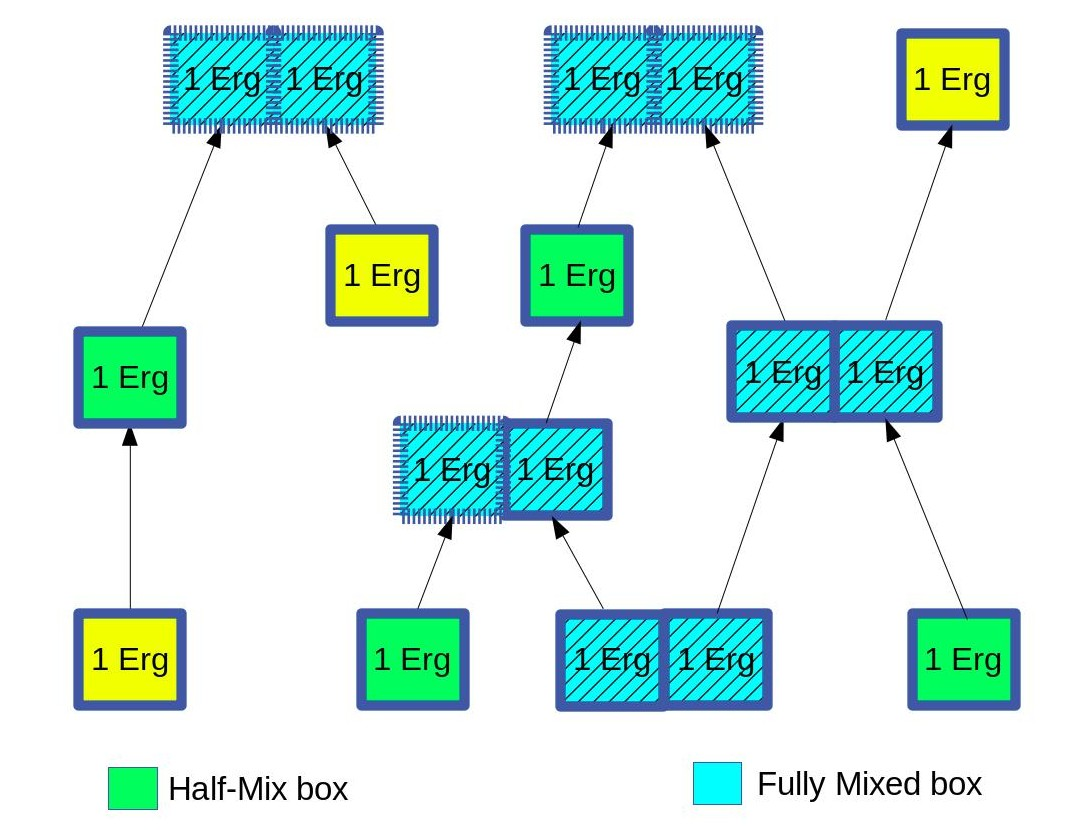
\includegraphics[width=\linewidth]{ErgoMix}
	\end{subfigure}
	\caption{Multi-round \algname}
\label{fig:mixname}
\end{figure}


\subsection{One \algname Round}
Each individual \algname round consists of two stages, the {\em pool} followed by the {\em mix} stage. 
Without loss of generality, Alice will pool and Bob will mix. 
Let $g$ be some generator of $G$ that is fixed beforehand. Each box is assumed to have two optional registers $\alpha, \beta$ that can store elements of $G$.

\begin{enumerate}
	\item \textbf{Pool:} To add a coin to the H-pool, Alice picks secret $x\in \mathbb{Z}_q$ and computes $u = g^x$. She then creates an output box $A$ protected by a script that requires the spending transaction to contain two output boxes $O_0, O_1$ satisfying the following conditions: 
	\begin{enumerate}
		\item Both contain the same value as $A$.
		\item Both are protected by the script: $$\texttt{proveDHTuple}(g, \alpha, u, \beta) \lor \texttt{proveDlog}(\beta)$$
        \item The registers $(\alpha, \beta)$ of $O_b$ and $O_{1-b}$ contain pairs $(c, d)$ and $(d, c)$ respectively for some $c, d\in G$. 
		\item One of $(g, u, c, d)$ or $(g, u, d, c)$ must be a valid Diffie-Hellman tuple, that is, of the form $(g, g^x, g^y, g^{xy})$. This is encoded %in \langname 
		as: $$\texttt{proveDHTuple}(g, u, c, d)\lor \texttt{proveDHTuple}(g, u, d, c)$$
	\end{enumerate}
	She waits for Bob to join the protocol, who will do so by spending $A$.


	\item \textbf{Mix:} Bob picks secrets $(b, y) \in \mathbb{Z}_2\times \mathbb{Z}_q$ and obtains $u$ from the script. He then computes $h= g^y$ and $v = u^y$. He spends $A$ with one or more of his own boxes to create two output boxes $O_0, O_1$ of equal value such that $O_b$ is spendable by Alice alone and $O_{1-b}$ by Bob alone:
	\begin{enumerate}
		\item Registers $(\alpha, \beta)$ of $O_b$ and $O_{1-b}$ store $(h, v)$ and $(v, h)$ respectively. 
		%		If the DDH problem in $G$ is hard, then given $(g, g^x)$ the distributions $({g}^{y}, {g}^{xy})$ and 
		%		$({g}^{xy}, {g}^{y})$ are computationally indistinguishable. In other words, without knowledge of $x$ or $y$, one cannot guess $b$ with probability better than $1/2$.
		\item $O_b, O_{1-b}$ are protected by the script: $$\texttt{proveDHTuple}(g, \alpha, u, \beta)\lor \texttt{proveDlog}(\beta)$$
		such that the box must be spent using a $\Sigma$-$\ornode$ proof (see Appendix~\ref{sigma-or}).
	\end{enumerate}
\end{enumerate}
After the mix, Alice and Bob can spent their respective boxes using their secrets. 
Alice can identify her box as the one with $\beta = \alpha^x$. 

\subsection{Analysis}

For correctness, Alice requires that she is always able to spend the coin. That is, Bob should not be able to spend $A$ in a manner that makes the resulting output(s) unspendable by Alice.

Let $x$ be the Alice's secret corresponding to her box $A$. First note that due to the clause 
\texttt{proveDHTuple($g, u, c, d$) || proveDHTuple($g, u, d, c$)}, Bob has no choice but to create two outputs $O_0, O_1$ such that the registers $(\alpha, \beta)$ of $O_b$ and $O_{1-b}$ contain $(g^y, g^{xy})$ and $(g^{xy}, g^y)$ respectively for some integer $y$ and bit $b$. This implies that that $O_b$'s spending condition reduces to:
$$\texttt{proveDHTuple}(g, g^{y}, g^x, g^{xy}) \lor \texttt{proveDlog}(g^{xy}).$$ 
The above statement can be proved by anyone who knows at least one of $x$ or $xy$. 
Thus, Alice can spend this because only she knows $x$. 

For soundness, Alice requires that no one else should be able to spend $O_b$, her Full-Mix box. Observe that the only way someone else could spend this box is by knowing $xy$, because they don't know $x$. Assume there is an algorithm that takes as input $g^x$ and somehow outputs $(g^y, g^{xy}, xy)$ for some $y \neq 0$. Then Alice can use this to immediately compute $y$, contradicting the fact that the discrete log problem in $G$ is hard. Thus, no one must know $xy$ and thereby, only Alice has the ability to spend $O_b$.

From Bob's point of view, the spending condition of $O_{1-b}$ reduces to 
$$\texttt{proveDHTuple}(g, g^{xy}, g^x, g^{y}) \lor \texttt{proveDlog}(g^{y}).$$
Since Bob knows $y$, he can spend the box using the right part of the statement. Finally, if someone apart from Bob spends $O_{1-b}$ then they must have used the left part of the statement because using the right part would required knowledge of $y$. However, using the left part is not possible because $(g, g^{xy}, g^x, g^{y})$ is not a valid DH Tuple. Hence, assuming that the original Schnorr proof is sound, no one else apart from Bob can spend $O_{1-b}$.

For privacy, the only difference between $O_b$ and $O_{1-b}$ is that $(g, \alpha, u, \beta)$ is a valid Diffie-Hellman tuple for $O_b$, while for $O_{1-b}$, the tuple is $(g, \beta, u, \alpha)$. Assuming that the Decision Diffie-Hellman (DDH) problem in $G$ is hard, no one apart from Alice or Bob has the ability to distinguish the boxes.
Thus, the boxes are indistinguishable before they are spent. To see that they remain so after being spent, observe that the protocol provides {\em spender indistinguishability} because each box is spent using a $\Sigma$-OR-proof that is zero-knowledge~\cite{Dam10}. 

\paragraph{Comparing with CoinJoin:} Referring to Section~\ref{coinjoin}, both CoinJoin and \algname use the technique of spending two boxes to create two indistinguishable boxes that provide the privacy. However, CoinJoin requires the owners of the two input boxes to perform an off-chain interaction over a private channel. In \algname, this interaction is replaced by a public transaction on the blockchain. While this adds one more transaction, it does not require interaction between the parties over a private channel. This makes \algname far more usable compared to CoinJoin. Note that \algname transactions are detectable, while CoinJoin transactions are indistinguishable from ordinary transactions.

\paragraph{Comparing with ZeroCoin:} Referring to Section~\ref{zerocoin}, both ZeroCoin and \algname use a pool (the H-pool in \algname and the U-pool in ZeroCoin). Additionally, both use zero-knowledge proofs to spend boxes from the pool in a way that hides the links between the outputs and the inputs, thereby providing the privacy. 
The difference is that the privacy in \algname is achieved in stages, two boxes at a time, while in ZeroCoin it is achieved in one stage. Secondly, the degree of privacy in ZeroCoin depends on the size of the U-pool, while that in \algname depends on the number of stages. Thirdly, the U-pool in ZeroCoin increases monotonically in size, since boxes are only added to it and never removed. The size of H-pool in \algname varies according to how many unspent Half-Mix boxes are present at any given time. Finally, the proof in ZeroCoin are quite large compared to those in \algname. The last two capture the main drawbacks of ZeroCoin that \algname addresses.
In particular, using \algname, we can obtain an equivalent (or sufficiently close) degree of privacy as from ZeroCoin without having to maintain the ever-increasing pools and with much shorter proofs. 

\paragraph{Offchain Pool:} The H-Pool can be kept entirely offchain, so that Alice's Half-Mix box need not be present on the blockchain till the time Bob decides to spend it. Alice sends her unbroadcasted transaction directly to Bob who will broadcast both transactions at some later time. 


\paragraph{Future enhancements:} Compared to CoinJoin, \algname requires an additional box -- the Half-Mix box -- as can be seen by by comparing Figures~\ref{fig:coinjoin} and~\ref{fig:mixname}. One way to eliminate the extra box would be to have the mix step output two indistinguishable Half-Mix boxes that can be used again in the mix step (or spent elsewhere). We could do this inefficiently by accumulating the statements and making the proof size proportional to the number of mixes. It is an open question if this can be done with a sublinear proof size.

\subsection{Implementing \algname In \langname}
\label{impl}
Each round of \algname is a two-stage protocol (pool followed by mix). One way to implement \algname would be to create a specialized blockchain just for this purpose that has the protocol hardwired (as was done in, for example, ZeroCash~\cite{zcash}). However, this limits the use of the blockchain. 

A more pragmatic approach would be to encode the protocol as a smart contract on top of a general-purpose blockchain. 
One such blockchain is Ergo~\cite{ergo}, whose scripting language \langname supports level C3 context (see Section~\ref{context}). Our example is implemented on top of Ergo~\cite{ergomix-impl}. 
The implementation uses the concepts from \cite{multistage} by encoding \algname as a two-stage protocol such that a `fingerprint' of the second stage is embedded within a smart contract from the first stage. 
In other words, Alice's box $A$ encodes the protocol by enforcing the structure of Bob's spending transaction. 
This is done as follows. For brevity, we will assume that \texttt{alpha}, \texttt{beta}, \texttt{gamma} are aliases for the first, second and third registers of a box that contain elements of $G$. The keywords \texttt{script} and \texttt{value} refer to the guard script (in binary format) and the quantity of primary tokens stored in the box. 

Let $x$ be Alice's secret and let $u = g^x$. To create the Half-Mix box with $u$, first define the script of the second stage, \texttt{fullMixScript} as:
{\small
\begin{Verbatim}[frame=single]
// Contract #1: contract for Full-Mix box (fullMixScript)
proveDHTuple(g, beta, alpha, gamma) || proveDlog(gamma)
\end{Verbatim}
}
Then compile the script and compute the hash of the result:

{\small
\begin{verbatim}
fullMixScriptHash = hash(compile(fullMixScript))
\end{verbatim}
}
Next create a script, \texttt{halfMixScript}, with the following code:
{\small
\begin{Verbatim}[frame=single]
// Contract #2: contract for Half-Mix box (halfMixScript)
INPUTS(0).id == id &&
OUTPUTS(0).beta == OUTPUTS(1).gamma && 
OUTPUTS(0).gamma == OUTPUTS(0).beta && 
OUTPUTS(0).alpha == alpha && OUTPUTS(1).alpha == alpha &&
OUTPUTS(0).value == value && OUTPUTS(1).value == value &&
hash(OUTPUTS(0).script) == fullMixScriptHash &&  
hash(OUTPUTS(1).script) == fullMixScriptHash &&
beta != gamma &&
(proveDHTuple(g, alpha, OUTPUTS(0).beta, OUTPUTS(0).gamma) || 
 proveDHTuple(g, alpha, OUTPUTS(0).gamma, OUTPUTS(0).beta))
\end{Verbatim}
}

Note that in \langname, \texttt{OUTPUTS(0)} is the first output of the spending transaction, \texttt{OUTPUTS(1)} is the second output, and so on. The keyword \texttt{id} refers to the globally unique identifier of the box. 

Alice's Half-Mix box $A$ is protected by \texttt{halfMixScript} given above. Alice must store $u$ in register \texttt{alpha} of that box.


\section{\mixname: \algname with Fee}
\label{fee}

Similar to ZeroCoin and CoinJoin (Figure~\ref{fig:coinjoin}), each Half-Mix and Full-Mix box in \algname must hold the same fixed value, which is carried over to the next stage. This implies zero-fee transactions because any fee must either be paid from the Full/Half-mix boxes (which breaks the fixed value requirement) or from a non-\algname box (which breaks privacy). Zero-fee transactions are fine in theory but not in practice. %Thus, any practical implementation of \algname must somehow handle fee. 

Here we describe how to handle fee on the Ergo blockchain. To differentiate the generic protocol (\algname) from the underlying implementation using Ergo, we give the name {\em \mixname} to any of the various extensions in this section that are largely specific to Ergo. 

We can classify \algname transactions into the following types:

\begin{enumerate}
    \item \textbf{Alice entry:} When someone plays the role of Alice to create a Half-Mix box (i.e., add a coin to the H-pool). The inputs to the transaction are one or more non-\mixname boxes ({\em external} boxes) and the output is one Half-Mix box. 
    \item \textbf{Bob entry:} When someone plays the role of Bob to spend a Half-Mix box (i.e., remove a coin from the H-pool). The other inputs of the transaction are one or more non-\mixname boxes and the outputs are two Full-Mix boxes. 
    \item \textbf{Alice or Bob exit:} When someone plays the role of Alice or Bob to spend a Full-Mix box and send the funds to a non-\mixname box (i.e., withdraw from the system). 
    \item \textbf{Alice or Bob reentry as Alice:} When someone plays the role of Alice or Bob to spend a Full-Mix box and create a Half-Mix box (i.e., send the coin back to the H-pool). The input is a Full-Mix box and the output is a Half-Mix box of the same amount.
    \item \textbf{Alice or Bob reentry as Bob:} When someone plays the role of Alice or Bob to spend a Full-Mix box along with another Half-Mix box and create two new Full-Mix boxes. The input is a Half-Mix box and a Full-Mix box and the outputs are two new Full-Mix boxes.
\end{enumerate}

These are depicted in Figure~\ref{fig:ergomixflow}.

\begin{figure}[h]
	\centering
	\begin{subfigure}{0.7\textwidth}
		\centering
		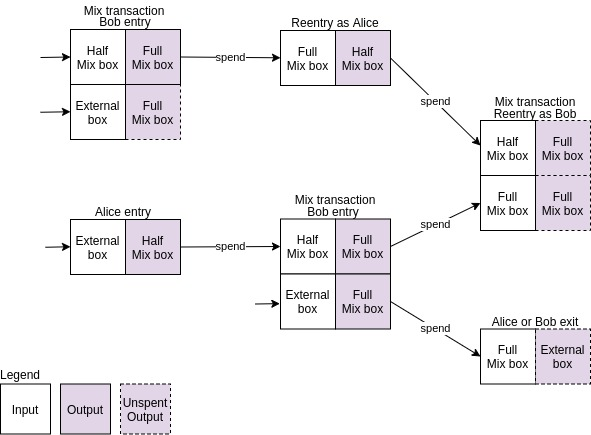
\includegraphics[width=\linewidth]{ErgoMixFlow.jpg}
	\end{subfigure}
	\caption{\algname Flow}
\label{fig:ergomixflow}
\end{figure}

Clearly, for both Alice and Bob entries, fee is not an issue because both parties can fund the fee component of the transaction from a known source, since these transactions are not meant to hide any information. Similarly for case 3, when exiting the system, part of the amount in the Full-Mix box can be used to pay fee. The only time we need to hide the source of fee is when we spend a Full-Mix box and want to reenter as either Alice or Bob. 

\subsection{An Altruistic Approach}
\label{donation}
% \subsection{Donation-Based Fee}

In this approach, fee is paid by a {\em sponsor} when spending a Full-Mix box for reentry. 
We use a variation of {\em Fee-Emission boxes} presented in~\cite{Fee-Emission}. 

\subsubsection{Fee-Emission Box}
A sponsor creates several Fee-Emission boxes to pay fee for spending full-mix boxes in the two reentry cases above. A Fee-Emission box can be spent under the following conditions:

\begin{enumerate}
    \item There is exactly one Fee-Emission box as input.
    \item There is exactly one Full-Mix box as input.
    \item Either exactly one input or exactly one output is a Half-Mix box.
    \item The updated balance is stored in a new Fee-Emission box.
\end{enumerate}

This is encoded in \langname as follows:

{\small
\begin{Verbatim}[frame=single]
// Contract #3: contract for Fee-Emission box
def isFull(b:Box) = hash(b.script) == fullMixScriptHash 
def isHalf(b:Box) = hash(b.script) == halfMixScriptHash
def isFee(b:Box) = hash(b.script) == feeScriptHash
def isCopy(b:Box) = b.script == script && 
                    b.value == value - fee
val asAlice = INPUTS.size == 2 && OUTPUTS.size == 3 &&
              isFull(INPUTS(0)) && isHalf(OUTPUTS(0)) &&
              isCopy(OUTPUTS(1)) && isFee(OUTPUTS(2)
val asBob = INPUTS.size == 3 && OUTPUTS.size == 4 &&
            isHalf(INPUTS(0)) && isFull(INPUTS(1)) &&
            isCopy(OUTPUTS(2)) && isFee(OUTPUTS(3))
asAlice || asBob 
\end{Verbatim}
}

The condition \texttt{asAlice} encodes the rules of spending a Full-Mix box to emulate Alice for the next mix and create a Half-Mix box. Similarly, the condition \texttt{asBob} has the rules for spending a Full-Mix box as Bob's contribution in a mix transaction. 

This approach is intended to encourage mixing because the sponsor pays the fee when a Full-Mix box is remixed. However, note that there is no guarantee that some given Full-Mix box was actually created in a mix transaction since one can create a box with the same structure that was not created in a mix transaction. The only way to distinguish such a box from a real one is to examine the transaction that created the box. However, this information is not available in \langname. Thus, the above approach is susceptible to freeloaders who store their funds in a Full-Mix box. However, such freeloaders cannot utilize the fee to send to anyone. They must either create a Half-Mix box or spend another Half-Mix box, thereby forcing them participate in the protocol. Consequently, there is no advantage to the freeloader because he still has to pay fee to create the fake full-mix box, which he could have used to participate in the mixing. Hence, we can safely ignore the freeloading attack. Note that there are ways, as shown later, to determine within \langname if the a Full-Mix box was created in a mix transaction.

The above approach requires someone to sponsor the mix transaction, which we call the {\em free system}. In practice we need \mixname to be self-sustaining that does not depend on sponsors, which we call the {\em paid system}. 
The following section will extend the free system to a paid system. 

\subsection{Mixing Tokens}

Ergo's primary token is known as {\em Erg}, which is necessary to pay for transaction fees and storage rent~\cite{chepurnoy2018systematic}. An Ergo transaction conserves primary tokens (they can neither be created nor destroyed) and any box must have a positive quantity of primary tokens.
Each box can optionally have {\em secondary tokens} which are uniquely identified by an id. Unlike primary tokens, an Ergo transaction can destroy secondary tokens. Additionally, each transaction can also create (i.e., {\em issue}) at most one new token in arbitrary quantity, whose id is the globally unique id of the first input box box of that transaction. 

In this approach, we will still use a Fee-Emission box (as in Section~\ref{donation}) to pay the fee in Ergs. However, we will also use secondary tokens issued by the creator of the Fee-Emission box, which we call {\em mixing tokens} (identified by \texttt{tokenId}). The Fee-Emission box can only be used by destroying a mixing token.

\subsubsection{Approximate Fairness}

We use the approximate fairness strategy described in~\cite{advtutorial}. At a high level the idea is as follows.
Each mix transaction consumes one mixing token, which must be supplied by the inputs. Thus, there must be at least one mixing token among the inputs. Additionally, to keep the outputs indistinguishable, each must have the same number of tokens. The approximate fairness strategy says that Bob must supply half the token, and is allowed to supply less tokens than Alice as long as both started with the same amount of tokens and Bob lost tokens in sequential mixes.

The approximate-fairness strategy works only if two conditions are satisfied. The first is that mixing tokens are confined within the system by restricting their transfer to only those boxes that participate in a remix. 
The second is to ensure that tokens always enter the system in a fixed quantity, and that too in one of the two \mixname boxes. 

\subsection{Token Confinement}

In this section we enforce the first requirement of approximate fairness, that of confining the tokens within the system. 
Recall that the Half-Mix box's script refers to the Full-Mix box's script via the constant \texttt{fullMixScriptHash}. Our approach additionally requires the Full-Mix box's script to refer back to the Half-Mix box's script. We do this by storing the hash of the Half-Mix script in one of the registers of the Full-Mix box. Let \texttt{delta} be an alias for this register that stores an array of bytes. The scripts are also modified.

\subsubsection{Fee-Emission Box}
We modify \texttt{isFull} method of the Fee-Emission box contract of Section~\ref{donation} as:

{\small
\begin{Verbatim}[frame=single]
// Contract #4: contract for Fee-Emission box
def isFull(b:Box) = hash(b.script) == fullMixScriptHash && 
                    b.delta == halfMixScriptHash
(... remaining code same as Contract #3)                    
\end{Verbatim}
}

Recall that the rule for spending the Fee-Emission box is to destroy one mixing token. While the above contract does not directly enforce this requirement, it does so indirectly via the Full-Mix and Half-Mix scripts discussed below.

\subsubsection{Full-Mix Box}

Modify \texttt{fullMixScript}, the contract of the Full-Mix box as follows: 
{\small
\begin{Verbatim}[frame=single]
// Contract #5: contract for Full-Mix box
def isHalf(b:Box) = hash(b.script) == delta && 
                    b.value == value
def isFull(b:Box) = b.script == script &&
                    b.delta == delta && b.value == value
def noToken(b:Box) = b.tokens(tokenId) == 0
val nextAlice = isHalf(OUTPUTS(0)) && INPUTS(0).id == id
val nextBob = isHalf(INPUTS(0)) && INPUTS(1).id == id
val destroyToken = OUTPUTS.forall(noToken)
val nextAliceLogic = OUTPUTS(0).tokens(tokenId) == 
                     INPUTS(0).tokens(tokenId) - 1 && 
                     OUTPUTS(0).tokens(tokenId) > 0

((nextAlice && nextAliceLogic) || nextBob || destroyToken) 
&& (... earlier condition from Contract #1)
\end{Verbatim}
}

The script enforces the transfer of mixing tokens when spending the Full-Mix box to create a Half-Mix box. In particular, the tokens can only be transferred if the transaction either outputs a Half-Mix box (i.e., the spender takes the role of Alice in the next mix step, in which case one mixing token is destroyed) or participates in a mix transaction as Bob and spends a Half-Mix box along with this Full-Mix box (in which case, the transfer of mixing tokens is governed by the contract in the Half-Mix box).
% The usage of mixing tokens when spending the Full-Mix box in a mix transaction is enforced in the Half-Mix box. In the remaining cases the mixing tokens must be destroyed.  

\subsubsection{Half-Mix Box}
Next, the Half-Mix box (\texttt{halfMixScript}) contract is also modified:
{\small
\begin{Verbatim}[frame=single]
// Contract #6: contract for Half-Mix box
val alice = INPUTS(0).tokens(tokenId)
val bob = INPUTS(1).tokens(tokenId)
val out0 = OUTPUTS(0).tokens(tokenId)
val out1 = OUTPUTS(1).tokens(tokenId)
val tLogic = alice + bob == out0 + out1 + 1 && bob > 0 && alice > 0 
  
OUTPUTS(0).delta == hash(script) && 
OUTPUTS(1).delta == hash(script) && out0 == out1 && tLogic &&
&& (... earlier condition from Contract #2)
\end{Verbatim}
}

The above contract assumes that the boxes already have some quantity of mixing tokens and enforces how these must be used. Each mix transaction is assumed to consume one such token, and to maintain privacy, the token balance must be equally distributed between the two outputs. The contract follows the {\em approximate-fairness} strategy where Alice requires Bob to contribute at least one mixing token~\cite{advtutorial}. It is possible to use {\em perfect fairness} by adding the condition \texttt{alice == bob}. 

Taken together, the contracts of the three boxes (Fee-Emission, Full-Mix and Half-Mix) {\em confine} the mixing tokens to the system, which comprises of sequential rounds of \mixname. In other words, once the mixing tokens have entered the system, they must remain within it. 

\subsection{Token Entry}

While the earlier section restricted how the mixing tokens are transferred after they are already in the system, this section will focus on defining how the tokens enter the system. This is done using a {\em Token-Emission box}. 

\subsubsection{Token-Emission Box}

A Token-Emission box is used for obtaining mixing tokens and gain entry into the system as either Alice or Bob. It contains the following contract. 

{\small
\begin{Verbatim}[frame=single]
// Contract #7: contract for Token-Emission box
def isCopy(b:Box) = b.script == script && b.value == value &&
                    b.tokens(tokenId) == tokens(tokenId) - amt
def isFull(b:Box) = hash(b.script) == fullMixScriptHash && 
                    b.delta == halfMixScriptHash
def isHalf(b:Box) = hash(b.script) == halfMixScriptHash
def isFee(b:Box) = hash(b.script) == feeScriptHash &&
                   b.value == fee
def isEntry(b:Box) = (isFull(b) || isHalf(b)) && 
                     b.tokens(tokenId) == amt
def isZero(b:Box) = b.tokens(tokenId) == 0

INPUTS(0).id == id && isZero(INPUTS(1)) && INPUTS.size == 2 &&
isEntry(OUTPUTS(0)) && isCopy(OUTPUTS(1)) && isFee(OUTPUTS(2))
\end{Verbatim}
}

% The Token-Emission box 
% is the final piece of the puzzle and 
% encodes the following logic. 
Anyone can spend the Token-Emission box to send a fixed amount \texttt{amt} of mixing tokens to either a Half-Mix box or a (fake) Full-Mix box, which should be the first output of the transaction. The other outputs are a copy of the token-emission box with the balance tokens and the fee paying output. The transaction must have exactly two inputs, with the token-emission box being the first and the second containing zero mixing tokens. 

We can use mixing tokens to verify that a given Full-Mix box was indeed created in a mix transaction, and a given Half-Mix box was indeed created by spending a Full-Mix box. In particular, this is true if and only if the box contains less than \texttt{amt} and more than 0 mixing tokens.  

While the above Token-Emission box gives the mixing tokens for free, it is trivial to modify the contract to sell the tokens at some given rate. The only change required is in the \texttt{isCopy} method:

{\small
\begin{Verbatim}[frame=single]
// Contract #8: contract for Token-Emission box
def isCopy(b:Box) = b.script == script && 
                    b.value == value + amt * rate &&
                    b.tokens(tokenId) == tokens(tokenId) - amt
(... remaining code same as Contract #7)
\end{Verbatim}
}

We also want the token issuer to be able to withdraw any Ergs deposited by token buyers. To achieve this, the token-emission box is again modified:

{\small
\begin{Verbatim}[frame=single]
// Contract #9: contract for Token-Emission box
(... earlier condition from Contract #8) || 
(issuerPubKey && INPUTS.size == 1 && 
 OUTPUTS(0).script == script && OUTPUTS(0).value > minErgs &&
 OUTPUTS(0).tokens(tokenId) == tokens(tokenId))
\end{Verbatim}
}
It is necessary to keep a certain amount of Ergs, \texttt{minErgs} inside each Token-Emission box, otherwise the box may be destroyed when miners collect storage rent. This value should be large enough to ensure sustenance for several years. 
In order to allow several people to buy tokens in the same block and to avoid collisions when multiple people try to spend the same token-emission box, there must be several token-emission boxes. 

\subsubsection{Analysis}

Because of the condition \texttt{bob > 0} in \texttt{tLogic} of the Half-Mix box, a mix transaction requires Bob to supply at least one token, and since these tokens can only be stored in either Full or Half-Mix boxes, the second input of a mix transaction must be a Full-Mix box (as opposed to any box).
That Full-Mix box can either be the output of a mix transaction (a real Full-Mix box) or the output of a token purchase transaction (a fake Full-Mix box).

Another consequence of \texttt{bob > 0} is that at least one token must exist in order to spend Alice's box. In the case that mixing tokens become unavailable, Alice's box is rendered unspendable. In order to handle this, we need to ensure that mixing tokens are always available. One way would be to have each token-emission box store a large number of tokens, much more than what can be purchased with all the available Ergs. Before storing any funds in a Half-Mix box, it must be ascertained that there are a large number of mixing tokens stored in at least one token-emission box. 

An alternate way to ensure that Alice's Half-Mix box does not get stuck due to non-availability of tokens would be to allow Alice to spend the box using her secret. This requires modifying the Half-Mix box as follows:

{\small
\begin{Verbatim}[frame=single]
// Contract #10: contract for Half-Mix box
def noToken(b:Box) = b.tokens(tokenId) == 0

(proveDlog(alpha) && INPUTS.size == 1 && OUTPUTS.forall(noToken)) || 
(... earlier condition from Contract #6)
\end{Verbatim}
}

The above modification allows Alice to spend the Half-Mix box using her secret but she must destroy all mixing tokens in doing so. 

Figure~\ref{fig:mixingtokens} gives an example flow with the above contracts in place. To avoid clutter, we skipped the fee output in the above flow. However, each transaction is implicitly assumed to have an additional box for paying fee.

\begin{figure}[h]
	\centering
	\begin{subfigure}{0.9\textwidth}
		\centering
		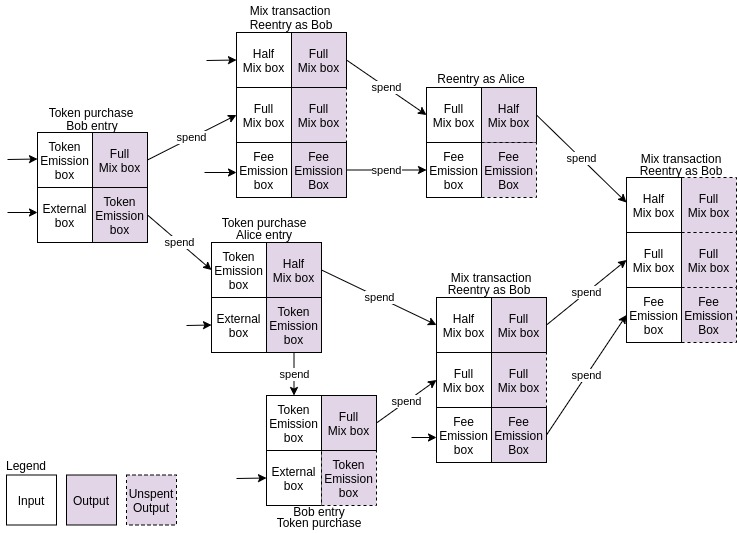
\includegraphics[width=\linewidth]{MixingTokens.jpg}
	\end{subfigure}
	\caption{Multi-round \mixname with Mixing Tokens to handle fee}
\label{fig:mixingtokens}
\end{figure}

Comparing this with Figure~\ref{fig:ergomixflow}, a mix transaction is always a reentry as Bob and both Alice and Bob's entry is through a token purchase transaction. 

The predicate \texttt{alice > 0} also requires that the Half-Mix box have at least one token, implying that the only way to create the Half-Mix box would be in a token purchase transaction or transaction for reentry as Alice. In particular, it is impossible to create a Half-Mix box in an other manner.

\subsubsection{Further Enhancements}


The approximate fairness approach requires each party to contribute half a mixing token in a mix transaction and the balance tokens are equally distributed among the parties, even if one supplied more. 

% Below we consider some enhancements to this. For brevity, we skip the \langname code and only give the high level approach. 

In the {\em First-Spender-Pays-Fee} approach, the idea is to benefit the party willing to wait longer and the party that spends their Full-Mix box first (retroactively) pays the fee for the mix transaction. This can be achieved as follows. Each mix transaction consumes two tokens. One is destroyed and the other is stored in a {\em refund box} that can be claimed by the second spender. We can identify the second spender as follows. 

\textbf{Identifying the second-spender:} Identifying if a given transaction is by the second spender is equivalent to determining if the other box is already spent. In a stateless language such as \langname, there is no direct way to determine if some other box is already spent. However, there are indirect ways and we describe one of them below. For brevity, we skip the \langname code and only give the high level approach. 

The protocol is modified to require each mix transaction to generate exactly 4 quantities of a new secondary token (with id $x$, determined as the id of the first input -- the Half-Mix box) distributed equally among 4 outputs. Two of these outputs are the standard Full-Mix output boxes $O_0, O_1$ with the additional spending condition that at least one output in the spending transaction must contain some non-zero quantity of token $x$. The other two outputs, $O_2, O_3$, have the following identical spending conditions:
\begin{enumerate}
	\item The sum of quantities of token $x$ in the inputs and outputs is 3 and 2 respectively.
	\item One output contains 2 quantities of token $x$ protected by the same script as this box. 
\end{enumerate}

It can be checked that the current spender is the second spender if and only if there is an input with two quantities of token $x$. The script also ensures that the first spender must create a new box with two tokens that can only be used by the second spender.

\section*{Acknowledgements}

We would like to thank anonymous developer {\em anon92048} for developing an implementation of the mixer, and also Jason Davies
for finding and reporting a vulnerability in both the paper and initial implementation. Vulnerability description made by Jason Davies
can be found in \cite{ergomix-vuln}.

% \section{Conclusion}
% [...]
\bibliographystyle{unsrt}
\bibliography{main}
\appendix

\section{$\Sigma$-Protocols}
\label{intro:sigma}
\algname uses Sigma protocols (written $\Sigma$-protocols), which are a generalization of the Schnorr identification scheme~\cite{Sch91}. 

\subsection{Schnorr Identification}
 Let $G$ be a cyclic multiplicative group of prime order $q$ and $g$ a generator of $G$. Alice wants to prove knowledge of some secret $x\in \mathbb{Z}_q$ to Bob who knows $u = g^x$. Assume that computing discrete logarithms in $G$ is hard. They perform the following protocol, also known as Schnorr identification:

\begin{enumerate}
	\item \textbf{Commit:} Alice selects random $r\in \mathbb{Z}_q$ and send $t = g^r\in G$ to Bob.
	\item \textbf{Challenge:} Bob selects random $c\in\mathbb{Z}_q$ and sends it to Alice.
	\item \textbf{Response:} Alice sends $z = r + cx$ to Bob, who accepts iff $g^z = t\cdot u^c$.
\end{enumerate}

The above protocol is a proof of knowledge because Bob can extract $x$ if he can get Alice to respond twice for the same $r$ and different $c$. As an example, for $c = 1, 2$, Bob can obtain $r+x$ and $r+2x$, the difference of which gives $x$. This is also called (special) soundness. The above protocol is also (honest verifier) zero-knowledge because anyone can impersonate Alice if the challenge $c$ of Step 2 is known in advance, simply by picking random $z \in\mathbb{Z}_q$ and computing $t = g^z/u^c$. The statement ``I know the discrete log of $u$ to base $g$'' is called the {\em proposition}, which we denote by $\tau$.

Any protocol that has the above 3-move structure (Alice $\stackrel{t}{\rightarrow}$ Bob, Bob $\stackrel{c}{\rightarrow}$ Alice, Alice $\stackrel{z}{\rightarrow}$ Bob), along with zero-knowledge and soundness property is called a $\Sigma$-protocol. 

For any $\Sigma$-protocol with messages $(t, c, z)$, we can apply the Fiat-Shamir transform~\cite{fiatshamir} to convert it into a non-interactive one by replacing the role of Bob in Step 2 by any hash function $H$ and computing $c$ = $H(t)$. The resulting protocol with messages $(t, H(t), z)$ can be performed by Alice alone. Intuitively, since $t$ fixes $c$, Bob cannot ``rewind'' Alice and get two different responses for the same $r$. Additionally, Alice cannot know $c$ in advance before deciding $t$ if $H$ behaves like a random oracle. We call such a non-interactive proof a {\em $\Sigma$-proof}~\cite{Cra96}. Conceptually, $\Sigma$-proofs are generalizations of digital signatures~\cite{CL06}.

\subsection{Composing $\Sigma$-Protocols}
\label{sigma-or}
Any two $\Sigma$-protocols of propositions $\tau_0, \tau_1$ with messages $(t_0, c_0, z_0), (t_1, c_1, z_1)$ respectively can be combined into a $\Sigma$-protocol of $\tau_0 \land \tau_1$ with messages $(t, c, z) = (t_0\Vert t_1,c_0\Vert c_1, c_0\Vert c_1)$. We call such a construction an $\andnode$ operator on the protocols. 
More interestingly, as shown in \cite{CDS94},the two protocols can also be used to construct a $\Sigma$-protocol for $\tau_0\lor \tau_1$, where Alice proves knowledge of the witness of one proposition, without revealing which. Let $b\in \{0, 1\}$ be the bit such that Alice knows the witness for $\tau_b$ but not for $\tau_{1-b}$. Alice will run the correct protocol for $\tau_b$ and a simulation for $\tau_{1-b}$. First she generates a random challenge $c_{1-b}$. She then generates $(t_{1-b}, z_{1-b})$ by using the simulator on $c_{1-b}$. She also generates $t_b$ by following the protocol correctly. The pair $(t_0, t_1)$ is sent to Bob, who responds with a challenge $c$. Alice then computes $c_b = c\oplus c_{1-b}$. She computes $z_b$ using $(t_b, c_b)$. Her response to Bob is $((z_0, c_0), (z_1, c_1))$, who accepts if: (1) $c = c_0 \oplus c_1$ and (2) $(t_0, c_0, z_0), (t_1, c_1, z_1)$ are both accepting conversations for $\tau_0, \tau_1$ respectively. We call such a construction a $\ornode$ operator. 

Clearly, both the $\andnode$ and $\ornode$ operators also result in $\Sigma$-protocols that can be further combined or made non-interactive via the Fiat-Shamir transform. Crucially, the proof for $\ornode$ does not reveal which of the relevant values the prover knows. For example, in \langname a ring signature by public keys $u_1, u_2$ can be specified as an $\ornode$ of $\Sigma$-protocols for proving knowledge of discrete logarithms of $u_1$ or $u_n$. The proof can be constructed with the knowledge of just one such discrete logarithm, and does not reveal which one was used in its construction. This is a crucial property used in \algname.
\langname, the programming language of Ergo gives the ability to build sophisticated $\Sigma$-protocols using the connectives $\andnode$, $\ornode$. This allows us to implement \algname on top of Ergo using smart contracts. 


\end{document}
